\documentclass[a4paper,12pt,danish]{article}

\usepackage[utf8]{inputenc}

\usepackage[english]{babel}

\usepackage{fixltx2e}

\usepackage{pgfplots, tikz}

\usepackage{graphicx}

\usepackage{lastpage}

\usepackage{fancyhdr}

\usepackage{multicol}

\usepackage{minted}

\usepackage[T1]{fontenc}

\usepackage[top=3cm, bottom=3cm, left=2.5cm, right=3.5cm]{geometry}

\usepackage{tocvsec2}

\usepackage{float}

\usepackage{tabularx}

\usepackage{parskip}

\usepackage{mathtools}

\usepackage{changepage}

\usepackage{gensymb}

\usepackage{mdwlist}

\usepackage{algorithm}

\usepackage{titlesec}

\usepackage{algpseudocode}

\usepackage{subfiles}

\usepackage{color}

\usepackage{booktabs}

%\usepackage{verbatim}

\usepackage[hidelinks]{hyperref}

\algrenewcommand\algorithmicprocedure{\textbf{function}}

\usepackage[nottoc,numbib]{tocbibind}

\usepackage{setspace}

\usepackage{array}

\usepackage{lastpage}
\pagestyle{fancy}

\cfoot{\thepage\ of \pageref{LastPage}}
\renewcommand{\headrulewidth}{0pt}
\fancyhead{}

\titlespacing*{\section}{0pt}{0.5cm}{0cm}
\titlespacing*{\subsection}{0pt}{0.3cm}{0cm}
\titlespacing*{\subsubsection}{0pt}{0.1cm}{0cm}
\titlespacing*{\paragraph}{0pt}{0cm}{0cm}

\setcounter{secnumdepth}{4}

\titleformat{\paragraph}
{\normalfont\normalsize\bfseries}{\theparagraph}{1em}{}


\title{\textbf{Algorithms and Datastructures -- AVL and Splay trees}}
\author{Stefan Ravn van Overeem – stvan13@student.sdu.dk \\
		Martin Staal Steenberg – mstee13@student.sdu.dk}

\begin{document}
\maketitle
\section{Implementation}
	We have implemented the Splay and AVL trees as classes, with the following functions: insert, contains and print.
	The trees also contains a pointer to the root node. The nodes have been implemented as a class as well containing the value, pointer to left and right child as well as the height of the node. The SplayNode also has a parent pointer, if the node is the root this pointer will be a null pointer.
	
\subsection{insert}
The insert function checks the value of the root node and compares it to the value we want to insert. If the value is larger than the node it goes to the right child else it goes to the left child. This is repeated until it finds a null pointer and the value is inserted.

\subsubsection*{AVL Tree}
The AVL tree does not insert the value if it is already contained in the tree. After the value have been inserted, the functions check if the height of one of the branches is above the allowed imbalance (1 in this case), if this is the case the tree is balanced.

\subsubsection*{Splay Tree}
After the value have been inserted the splay tree, splays the inserted value up to the root node, using the Zig, Zag, ZigZig, ZigZag, ZagZag and ZagZig function.

\subsection{contains}
The contains function checks the value of the root node and compares it to the value we want to find. If the value is larger than the node it goes to the right child else it goes to the left child. This is repeated until it either finds the value and true is returned or it reaches a null pointer false is returned.

\subsubsection*{Splay Tree}
The splay tree then splays the value to the root node.

\subsection{print}
The print function prints the value of the root node then it goes down the left and right branch recursively. This is repeated until it reaches a null pointer.

\section{Time Complexity}

\begin{figure}[H]
\centering
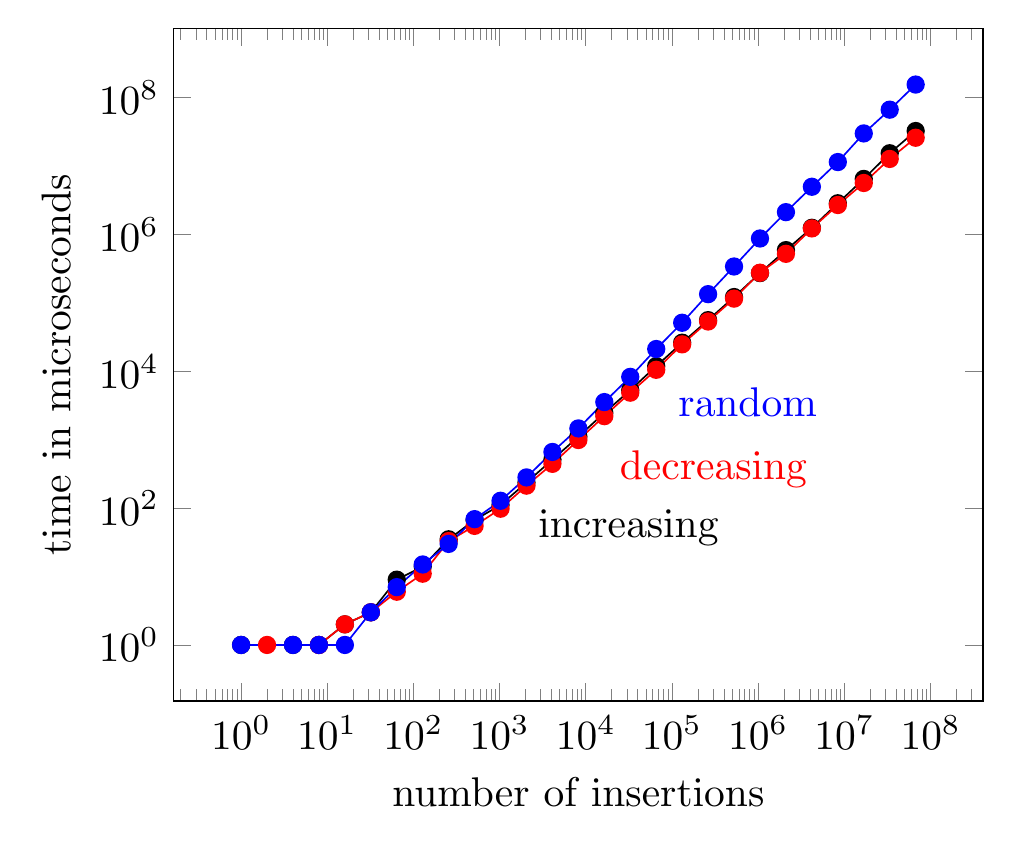
\begin{tikzpicture} [scale=1.5, transform shape]
\begin{axis}[
xmode=log,
ymode=log,
scatter/classes={a={mark=o,draw=black}},
xlabel = {number of insertions},
ylabel = {time in microseconds}
    ]
\addplot[scatter]
table[meta=label] {
x y label
1	1 a
2	0 a
4	1 a
8	1 a
16	2 a
32	3 a
64	9 a
128	14 a
256	35 a
512	67 a
1024	111 a
2048	237 a
4096	511 a
8192	1107 a
16384	2470 a
32768	5305 a
65536	11891 a
131072	26178 a
262144	55941 a
524288	121713 a
1048576	272814 a
2097152	590456 a
4194304	1252226 a
8388608	2857436 a
16777216	6489542 a
33554432	15388861 a
67108864	32523348 a
    } node[right,pos=0.3, xshift = 0.5 cm] {increasing};
\addplot[scatter, color=red]
table[meta=label] {
x y label
1	0 a
2	1 a
4	0 a
8	1 a
16	2 a
32	3 a
64	6 a
128	11 a
256	33 a
512	55 a
1024	98 a
2048	213 a
4096	444 a
8192	990 a
16384	2209 a
32768	4868 a
65536	10514 a
131072	24773 a
262144	53414 a
524288	115341 a
1048576	276034 a
2097152	521372 a
4194304	1225667 a
8388608	2696165 a
16777216	5658867 a
33554432	12705332 a
67108864	25937929 a
    } node[right,pos=0.4, xshift = 0.5 cm] {decreasing};
    \addplot[scatter, color=blue]
table[meta=label] {
x y label
1	1 a
2	0 a
4	1 a
8	1 a
16	1 a
32	3 a
64	7 a
128	15 a
256	30 a
512	69 a
1024	128 a
2048	281 a
4096	662 a
8192	1462 a
16384	3548 a
32768	8284 a
65536	21169 a
131072	51246 a
262144	134126 a
524288	340354 a
1048576	873544 a
2097152	2119636 a
4194304	4979764 a
8388608	11445645 a
16777216	29994571 a
33554432	66714828 a
67108864	155453243 a
    } node[right,pos=0.5, xshift = 0.5 cm] {random};

\end{axis}
\end{tikzpicture}
\caption{AVLTree insertion tests, double logarithmic plot}
\label{avl}
\end{figure}


\begin{figure}[H]
\centering
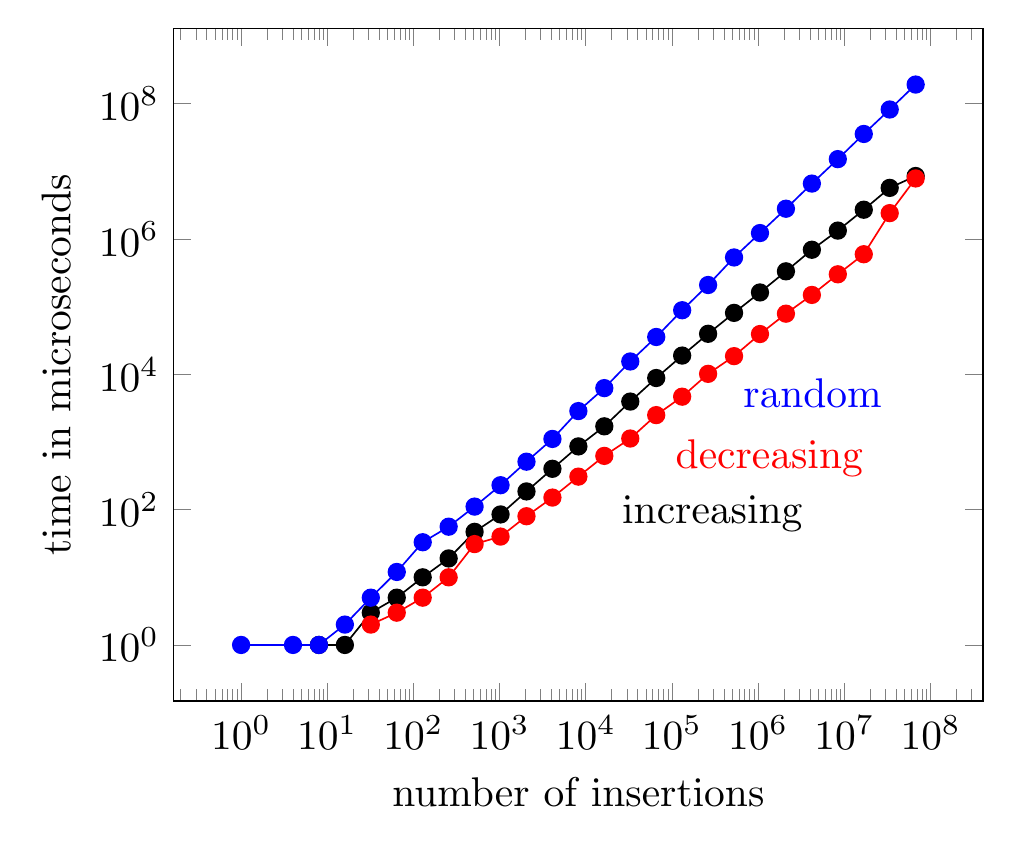
\begin{tikzpicture} [scale=1.5, transform shape]
\begin{axis}[
xmode=log,
ymode=log,
scatter/classes={a={mark=o,draw=black}},
xlabel = {number of insertions},
ylabel = {time in microseconds}
    ]
\addplot[scatter]
table[meta=label] {
x y label
1	0 a
2	0 a
4	0 a
8	1 a
16	1 a
32	3 a
64	5 a
128	10 a
256	19 a
512	47 a
1024	85 a
2048	186 a
4096	402 a
8192	862 a
16384	1707 a
32768	3968 a
65536	8842 a
131072	18981 a
262144	39836 a
524288	81169 a
1048576	162766 a
2097152	334026 a
4194304	696276 a
8388608	1336262 a
16777216	2720356 a
33554432	5722003 a
67108864	8571887 a
    } node[right,pos=0.3, xshift = 0.9 cm] {increasing};
\addplot[scatter, color=red]
table[meta=label] {
x y label
1	0 a
2	0 a
4	0 a
8	0 a
16	0 a
32	2 a
64	3 a
128	5 a
256	10 a
512	31 a
1024	40 a
2048	80 a
4096	151 a
8192	308 a
16384	624 a
32768	1127 a
65536	2501 a
131072	4683 a
262144	10186 a
524288	18617 a
1048576	39499 a
2097152	79020 a
4194304	149598 a
8388608	301885 a
16777216	597631 a
33554432	2422120 a
67108864	7886538 a
    } node[right,pos=0.4, xshift = 0.5 cm] {decreasing};
    \addplot[scatter, color=blue]
table[meta=label] {
x y label
1	1 a
2	0 a
4	1 a
8	1 a
16	2 a
32	5 a
64	12 a
128	33 a
256	56 a
512	111 a
1024	230 a
2048	512 a
4096	1111 a
8192	2869 a
16384	6268 a
32768	15525 a
65536	35739 a
131072	88864 a
262144	209742 a
524288	535698 a
1048576	1229379 a
2097152	2813989 a
4194304	6624778 a
8388608	15231607 a
16777216	35881712 a
33554432	82490657 a
67108864	192958080 a
    } node[right,pos=0.5, xshift = 1.1 cm] {random};

\end{axis}
\end{tikzpicture}
\caption{SplayTree insertion tests, double logarithmic plot}
\label{splay}
\end{figure}
		
As can be seen on figure \ref{avl} and \ref{splay} the time complexity of both the AVL and Splay tree for $\mathcal{N}$ insertions is $\mathcal{O(N \cdot \log N)}$. This is in agreement with the theory.

The memory complexity of both the AVL and Splay implementation is $\mathcal{O(N)}$ because the only thing that have to be stored is the call stack and the nodes.

\section{Sample Print}
Examples of the AVL and Splay trees print function with 10 nodes. 
\begin{figure}[H]
\centering
\begin{tabular}{|c|c|c|c|c|c|c|c|c|c|}
  \hline
  66 & 6 & 78 & 49 & 14 & 45 & 90 & 5 & 17 & 19 \\
  \hline 
\end{tabular}
\caption{sample input}
\end{figure}

\begin{figure}[H]
\centering
\begin{tabular}{|c|c|}
  \hline
  AVLTree & SplayTree \\
  \hline
  49 & 19 \\
  \hline
  14 & 17 \\
  \hline
  6 & 5 \\
  \hline
  5 & 14 \\
  \hline
  19 & 6 \\
  \hline
  17 & 45 \\
  \hline
  45 & 90 \\
  \hline
  78 & 78 \\
  \hline
  66 & 49 \\
  \hline
  90 & 66 \\
  \hline 
\end{tabular}
\caption{sample output}
\end{figure}

\section{Code}
\subsection*{AVLTree.hpp}
\inputminted[frame=bottomline, linenos, breaklines]{cpp}{"../code/headers/AVLTree.hpp"}

\subsection*{AVLTree.tpp}
\inputminted[frame=bottomline, linenos, breaklines]{cpp}{"../code/headers/AVLTree.tpp"}

\subsection*{SplayTree.hpp}
\inputminted[frame=bottomline, linenos, breaklines]{cpp}{"../code/headers/SplayTree.hpp"}

\subsection*{SplayTree.tpp}
\inputminted[frame=bottomline, linenos, breaklines]{cpp}{"../code/headers/SplayTree.tpp"}

\subsection*{test.cpp}
\inputminted[frame=bottomline, linenos, breaklines]{cpp}{"../code/sources/test.cpp"}

\end{document}
